\subsection{Теоретическая оценка значения \texorpdfstring{$\kappa$}{kappa}}

Оценим значение параметра $\kappa$:
\begin{equation*}
    \kappa = \sigma_0 n l \sqrt{\frac{m}{2 \pi \sub{k}{B} T}},
\end{equation*}
или, можем переписать в виде
\begin{equation*}
    \kappa = \frac{\sigma_0 n l}{v_0 \sqrt{\pi}}, \hspace{10 mm} v_0 = \sqrt{\frac{2 \sub{k}{Б} T}{m}}.
\end{equation*}

\textbf{Концентрация}. Концентрацию атомов лития ${}^7$Li можем найти, зная зависимость \cite{phd_mahalov} давления насыщенных паров $P$ от температуры $T$:
\begin{equation*}
    P[T] = 133.32 \times \exp\left[\ln 10 \left(
                10.3354 - \frac{8345.57}{T} - 8.84 \times 10^{-5} T - 0.68106 \log_{10} [T]
            \right)\right].
\end{equation*}
Тогда, например, при температуре $T = 300+273$ K, 
\begin{equation*}
    P[573 \, \text{K}] = 9.5 10^{-5} \ \text{Па},
    \hspace{0.5cm} \Rightarrow \hspace{0.5cm}
    n[573 \, \text{K}] = \frac{P}{\sub{k}{Б} T} = 1.2 \times  10^{-16} \ \text{м}^{-3}.
\end{equation*}

\textbf{Сечение}. Сечение рассеяние для двухуровневой системы ($\lambda = 671$ нм)  
\begin{equation*}
    \sigma_0^{\text{теор}} = \frac{3 \pi}{8} \lambda^2 \approx 5.3 \times 10^{-13} \ \text{м}^2.
\end{equation*}
% \red{уточнить, указать источник}.

Итого, для $l = 10$ см, при температуре в $300\ {}^{\circ}$С, для ${}^7$Li находим
\begin{equation*}
    \kappa = 0.31 \frac{1}{\text{м}/\text{с}},
    \hspace{5 mm} 
    v_0 = 1.2 \times 10^3 \ \text{м}/\text{с},
    \hspace{10 mm} 
    \sigma_0 n l = 6.4 \times 10^2.
\end{equation*}


\subsection{Количественная картинка}

Подставляя найденное в предыдущем разделе значение $\kappa$ в формулу \eqref{maineq}, получаем общий вид спектроскопии: рис. \ref{fig:frac12}.

\begin{figure}[h]
    \centering
    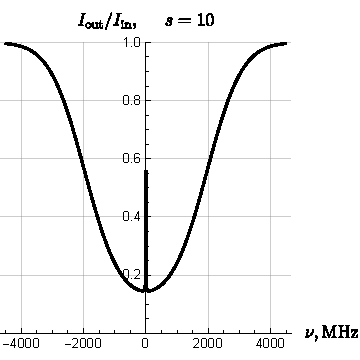
\includegraphics[width=0.3\textwidth]{"D:\\Kami\\git_folder\\notes_5sem\\rqc\\saturation_spectr_simulation\\frac2.pdf"}
    \hspace{5 mm} 
    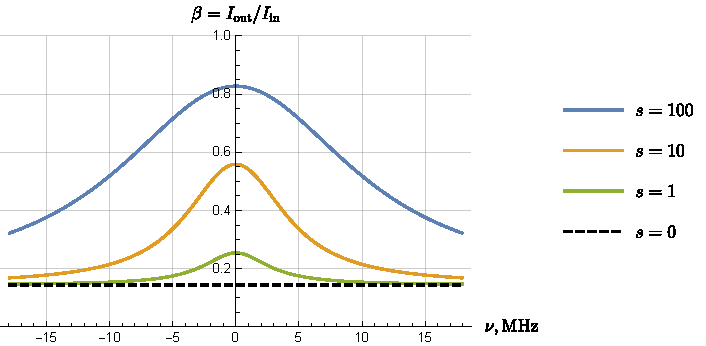
\includegraphics[width=0.6\textwidth]{"D:\\Kami\\git_folder\\notes_5sem\\rqc\\saturation_spectr_simulation\\frac1.pdf"}
    \caption{Оценка $\beta$ вблизи резонанса при температуре в $300\ {}^{\circ}$С для $\sigma_0^{\text{теор}}$ и $l = 10$ см}
    \label{fig:frac12}
\end{figure}


Заметим, что указанные параметры системы приводят к значению $\beta$ в резонансе при $s=0$:
\begin{equation*}
    \beta[s=0, \nu=\nu_0] = e^{- \kappa F(0)} = 0.14,
\end{equation*}
что похоже на правду (см. раздел ...).





\newpage

\subsection{Оценка контрастности по наблюдаемой глубине доплеровского провала}

В первом приближении, не зная значения $\kappa$, можем оценить его, зная глубину доплеровского провала в резнансе $\nu_0$. Введем для удобства приведенную интенсивность $\beta \overset{\mathrm{def}}{=}  \sub{I}{out}/\sub{I}{in}$, далее в этом разделе всегда полагаем $\nu = \nu_0$, тогда
\begin{equation*}
    \beta(s=0) \overset{\mathrm{def}}{=}  \beta_0 = e^{- \kappa F(0)},
    \hspace{0.5cm} \Rightarrow \hspace{0.5cm}
    \kappa = \frac{\ln 1/\beta_0}{F(0)},
\end{equation*}
где $1-\beta_0$ -- глубина доплеровского провала.

Тогда контрастность спектроскопии $K$, определенную, как отношение высоты лэмбоского пика к глубине доплеровского провала, можем найти, как
\begin{equation*}
    K(s) = \frac{e^{-\kappa F(s)}-e^{-\kappa F(0)}}{1-e^{-\kappa F(0)}} = 
    \frac{\beta_0^{F(s)/F(0)}-\beta_0}{1-\beta_0}.
\end{equation*}
Ниже на рисунке приведены значения контрастности $K(s)$ для различных $\beta$.

\begin{figure}[h]
    \centering
    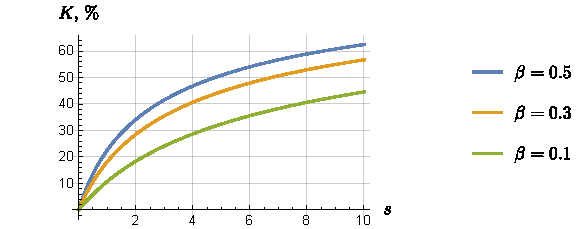
\includegraphics[width=0.65\textwidth]{"D:\\Kami\\git_folder\\notes_5sem\\rqc\\saturation_spectr_simulation\\K.pdf"}
    \caption{Оценка контрастности при различных значениях $\beta$, как функция от $s$}
    %\label{fig:}
\end{figure}



\subsection{Сравнение теоретической и экспериментальной оценки \texorpdfstring{$\kappa$}{kappa}}

Пока что, в контексте выбранной модели, хуже всего можем оценить $l$, поэтому будем сравнивать теоритескую и экспериментальную оценку $\kappa$ по значению $l$  при котором они бы сходились:
\begin{equation*}
    l = \underbrace{\frac{\log 1/\beta_0}{F[0, \nu_0]}}_{\kappa} \frac{\sqrt{\pi}}{n \sigma_0} \underbrace{\sqrt{\frac{2 \sub{k}{Б} T}{m}}}_{v_0}.
\end{equation*}
Считая $\sigma_0 = \sigma_0^{\text{теор}}$, построим зависимость $l[\beta]$, рис. \ref{fig:lx}.

\begin{figure}[h]
    \centering
    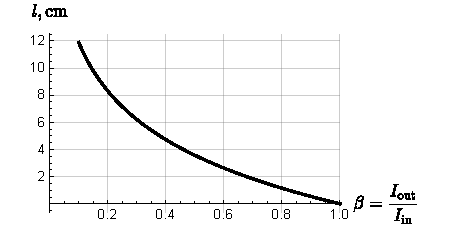
\includegraphics[width=0.5\textwidth]{"D:\\Kami\\git_folder\\notes_5sem\\rqc\\saturation_spectr_simulation\\lx.pdf"}
    \caption{Оценка длины взаимодействия лазера с литием при температуре в $300\ {}^{\circ}$С}
    \label{fig:lx}
\end{figure}
